% This template has been tested with LLNCS DOCUMENT CLASS -- version 2.20 (24-JUN-2015)

%"runningheads" enables:
%  - page number on page 2 onwards
%  - title/authors on even/odd pages
%This is good for other readers to enable proper archiving among other papers and pointing to
%content. Even if the title page states the title, when printed and stored in a folder, when
%blindly opening the folder, one could hit not the title page, but an arbitrary page. Therefore,
%it is good to have title printed on the pages, too.
\documentclass[runningheads,a4paper]{llncs}[2015/06/24]

\makeatletter
\renewcommand\paragraph{\@startsection{paragraph}{4}{\z@}%
            {-2.5ex\@plus -1ex \@minus -.25ex}%
            {1.25ex \@plus .25ex}%
            {\normalfont\normalsize\bfseries}}
\makeatother
\setcounter{secnumdepth}{2} % how many sectioning levels to assign numbers to
\setcounter{tocdepth}{4}    % how many sectioning levels to show in ToC

%cmap has to be loaded before any font package (such as cfr-lm)
\usepackage{cmap}
\usepackage[T1]{fontenc}

\usepackage{graphicx}
\graphicspath{ {images/} }

%Even though `american`, `english` and `USenglish` are synonyms for babel package (according to https://tex.stackexchange.com/questions/12775/babel-english-american-usenglish), the llncs document class is prepared to avoid the overriding of certain names (such as "Abstract." -> "Abstract" or "Fig." -> "Figure") when using `english`, but not when using the other 2.
%english has to go last to set it as default language
\usepackage[ngerman,english]{babel}
%Hint by http://tex.stackexchange.com/a/321066/9075 -> enable "= as dashes
\addto\extrasenglish{\languageshorthands{ngerman}\useshorthands{"}}

%better font, similar to the default springer font
%cfr-lm is preferred over lmodern. Reasoning at http://tex.stackexchange.com/a/247543/9075
\usepackage[%
rm={oldstyle=false,proportional=true},%
sf={oldstyle=false,proportional=true},%
tt={oldstyle=false,proportional=true,variable=true},%
qt=false%
]{cfr-lm}
%
%if more space is needed, exchange cfr-lm by mathptmx
%\usepackage{mathptmx}

%for demonstration purposes only
\usepackage[math]{blindtext}

%Sorts the citations in the brackets
%It also allows \cite{refa, refb}. Otherwise, the document does not compile.
%  Error message: "White space in argument"
\usepackage{cite}
\usepackage[mathletters]{ucs}
\usepackage[utf8x]{inputenc}

\usepackage{amsmath}
\usepackage{algorithm}
\usepackage[noend]{algpseudocode}

\makeatletter
\def\BState{\State\hskip-\ALG@thistlm}
\makeatother


%% If you need packages for other papers,
%% START COPYING HERE
%% COPY ALSO cmap and fontenc from lines 10 to 12

%extended enumerate, such as \begin{compactenum}
\usepackage{paralist}

%put figures inside a text
%\usepackage{picins}
%use
%\piccaptioninside
%\piccaption{...}
%\parpic[r]{\includegraphics ...}
%Text...

%for easy quotations: \enquote{text}
\usepackage{csquotes}

%enable margin kerning
\usepackage{microtype}

%tweak \url{...}
\usepackage{url}
%\urlstyle{same}
%improve wrapping of URLs - hint by http://tex.stackexchange.com/a/10419/9075
\makeatletter
\g@addto@macro{\UrlBreaks}{\UrlOrds}
\makeatother
%nicer // - solution by http://tex.stackexchange.com/a/98470/9075
%DO NOT ACTIVATE -> prevents line breaks
%\makeatletter
%\def\Url@twoslashes{\mathchar`\/\@ifnextchar/{\kern-.2em}{}}
%\g@addto@macro\UrlSpecials{\do\/{\Url@twoslashes}}
%\makeatother

%diagonal lines in a table - http://tex.stackexchange.com/questions/17745/diagonal-lines-in-table-cell
%slashbox is not available in texlive (due to licensing) and also gives bad results. This, we use diagbox
%\usepackage{diagbox}

%required for pdfcomment later
\usepackage{xcolor}


%enable nice comments
%this also loads hyperref
\usepackage{pdfcomment}
%enable hyperref without colors and without bookmarks
\hypersetup{hidelinks,
   colorlinks=true,
   allcolors=black,
   pdfstartview=Fit,
   breaklinks=true}
%enables correct jumping to figures when referencing
\usepackage[all]{hypcap}

\newcommand{\commentontext}[2]{\colorbox{yellow!60}{#1}\pdfcomment[color={0.234 0.867 0.211},hoffset=-6pt,voffset=10pt,opacity=0.5]{#2}}
\newcommand{\commentatside}[1]{\pdfcomment[color={0.045 0.278 0.643},icon=Note]{#1}}

%compatibality with packages todo, easy-todo, todonotes
\newcommand{\todo}[1]{\commentatside{#1}}
%compatiblity with package fixmetodonotes
\newcommand{\TODO}[1]{\commentatside{#1}}

%enable \cref{...} and \Cref{...} instead of \ref: Type of reference included in the link
\usepackage[capitalise,nameinlink]{cleveref}
%Nice formats for \cref
\crefname{section}{Sect.}{Sect.}
\Crefname{section}{Section}{Sections}

\usepackage{xspace}
%\newcommand{\eg}{e.\,g.\xspace}
%\newcommand{\ie}{i.\,e.\xspace}
\newcommand{\eg}{e.\,g.,\ }
\newcommand{\ie}{i.\,e.,\ }

%introduce \powerset - hint by http://matheplanet.com/matheplanet/nuke/html/viewtopic.php?topic=136492&post_id=997377
\DeclareFontFamily{U}{MnSymbolC}{}
\DeclareSymbolFont{MnSyC}{U}{MnSymbolC}{m}{n}
\DeclareFontShape{U}{MnSymbolC}{m}{n}{
    <-6>  MnSymbolC5
   <6-7>  MnSymbolC6
   <7-8>  MnSymbolC7
   <8-9>  MnSymbolC8
   <9-10> MnSymbolC9
  <10-12> MnSymbolC10
  <12->   MnSymbolC12%
}{}
\DeclareMathSymbol{\powerset}{\mathord}{MnSyC}{180}

% correct bad hyphenation here
\hyphenation{op-tical net-works semi-conduc-tor}

%% END COPYING HERE


\begin{document}

\title{Ensemble Method for Time Series Forecasting}
%If Title is too long, use \titlerunning
%\titlerunning{Short Title}

%Single insitute
\author{Aleksandar Bachvarov \and Atanas Dimitrov}
%If there are too many authors, use \authorrunning
%\authorrunning{First Author et al.}
\institute{
Karlsruhe Institute of Technology\\
\email{aleksandar.bachvarov@gmail.com}, \email{atanas\_sz@abv.bg}
}

%Multiple insitutes
%Currently disabled
%
\iffalse
%Multiple institutes are typeset as follows:
\author{Firstname Lastname\inst{1} \and Firstname Lastname\inst{2} }
%If there are too many authors, use \authorrunning
%\authorrunning{First Author et al.}

\institute{
Insitute 1\\
\email{...}\and
Insitute 2\\
\email{...}
}
\fi
			
\maketitle

\begin{abstract}
Time series forecasting is an important field of study in the machine learning. It's influential in the modern insecure world, for it gives approximated data of future events (e.g. vulcanic eruption, birth and death rate estimation, demand for energy), which leads to proper preparations for them. In this paper an innovative ensemble method for time series forecasting is introduced, as well as the time series forecasting evolution throughout history and its machine learning background. The method is based on an ensemble strategy that combines arbitrated by a meta-learning model forecasters. The model is dynamically adapting over time by being constantly fed with new data, which improves the accuracy of the predictions and the overall performance.
\end{abstract}

\begin{keywords}
time series, forecasting, ensemble methods, machine learning, arbitrating  
\end{keywords}


\section{Introduction}\label{sec:intro}
This paper is the essential part of a seminar work related to Mobile Computing with particular topic \enquote{Ensemble Method for Time Series Forecasting}. It's an assignment in our B.Sc. Computer Science studies at Karlsruhe Institute of Technology. We chose the topic for a number of reasons: One of our personal interests are finance and stock trading. Hence, as the stock prices (and prices at all) are time series, we wanted to dive into the topic of time series predicting tasks and doing so to educate ourselves about financial assets price forecasting. Secondly, the topic is narrowly connected with machine learning - a field of computer science with great significance and endless potential, in which we are motivated to develop ourselves. Through our researches we will get to know more or less its basics.       

\section{Fundamentals of time series forecasting}

	\subsection{Definition}
		\subsubsection{Time series}
		 \hspace{1cm}\\\\A time series is sequence of data points, which are ordered and indexed by time. The data presented in the series could be any variable capable for observation over time. Some examples of time series include the price of a specific stock, the height level of a river and the national birth rate over time. Time series could be presented by multiple ways: as a list of values, as a graph, as a bar chart etc. On  \hyperref[fig:bitcoin]{Fig. \ref{fig:bitcoin}} you can see a graph of the bitcoin price time series over the last year. Besides in investing, time series is used in many other fields like e.g. statistics, insurance, weather forecasting, astronomy, applied  science etc.
		
\begin{figure}[h]
\centering

\includegraphics[width=\textwidth]{bitcoin}
\caption{Bitcoin price history from December,  2016 to December, 2017.}
\label{fig:bitcoin}
\end{figure}

		\subsubsection{Forecasting} \hspace{1cm}\\\\Time series forecasting represents the process of predicting the future values of the observed variable based on the already available data. In order to achieve that, dependencies among the available time series must be found, which then approximate the possible future values. Various methods were used over the years. They are in general divided  in two groups: linear and non-linear methods. The most significant of them will be wider presented  further in this paper. It's important to be noted that time series forecasting is just forecasting - the purpose is that the forecast is as close as possible to the future value, but there is no warranty for that. Generally the deviation of the forecast increases with his time distance.\\\\ Time series could be non-stationary (volatile) or stationary. In other words - to have higher or lower degree of stationarity. It appears that the distribution of the stationary one depends much more on a long term trend while the distribution of the not-stationary one - on occasional events. Example for an extremely stationary time series is the coin flipping over time, example for an extremely volatile one - the bitcoin price. Because of its characteristics the volatile time series is much harder to predict. Its wide spread and importance led to the development of more complex (non-linear) methods for doing that. Those methods include and are based on some machine learning techniques like e.g. bagging and boosting and also on key machine learning tools like artificial neural networks. Time series forecasting is one of the classic and at the same time very important areas of the machine learning.
	\subsection{Origins and related topics}
		\subsubsection{Machine Learning}\hspace{1cm}\\\\ 
In the recent years, as many useful applications of machine learning have been developed and have become part of our everyday life, its significance increased. We hear more and more often the term on the news or read about it on the Internet. In many cases machine learning is used as a synonym for artificial intelligence (AI), which is inexact. AI is field of computer science, which is studying and  applying approaches for making computers being able to execute cognitive tasks\cite{AIvsML}. Machine learning is one of those approaches and it's by far the most successful (widely used, with the most applications) one of them\cite{quinlan1986induction}. Its subject is the studying and the computer modelling of learning processes.\cite{Michalski1983}. \\\\ One common way to create a new machine learning process is to research the human learning mechanisms, to adapt them and then accordingly to simulate them  with algorithms. The artificial neural networks (commonly utilized machine learning tool) are example for that and they will be discussed thoroughly further in the paper. It is  restrictive to believe that the learning patterns that come from the nature are the only possible way for acquiring knowledge. Reserchers also try to manifacture their own ones. By doing this main criteria are the methods'  generality and performance rather than their psychological explanation\cite{Michalski1983}.\\\\ 
In order to better understand one single learning methodology, we classify it by some meaningful parameters:
\begin{enumerate}
\item the amount of inference performed on the available information
\item the representation of knowledge acquired by the learner. 
\item the application domain of the collected knowledge 
\end{enumerate}\hspace{1cm}\\Different amount of inference means that the learning system analyses the data more or less and makes more or less interdependencies between it. Example for no inference is the simple remembering of facts with no thoughts about them and any other already existing knowledge. Example for middle range inference is the learning from teacher or book that provides the learner positive and negative examples. The learner analyses the input data and makes some conclusion about it based mainly on its already existing knowledge. Example for extremely high level of inference is the learning from observation and the discovery. There is no source of certain information to learn from and the learner should discover it alone\cite{Michalski1983}. The high and the low level of inference of learning methods has both their pluses and minuses - it's much harder and slower to learn something single-handed, but because of that you reach deeper understanding of the topic.\\\\
There are a lot of different representations of knowledge that the learner can produce. Some popular examples include the decision trees that will be discussed in detail, parameters in algebraic expressions, formal grammars, graphs, computer programs, classification categories etc.\\\\
We know from the near past and the present  (and for sure will hear more about it in the future) that the machine learning has a lot of applications. Some popular application domains are the self driving cars, speech and face recognition, the expert systems and of course - the subject of our paper - time series forecasting.  \\\\As next on this paper follow some presentation of key tools and techniques in machine learning at all and in the field of time series forecasting specifically.
				
\paragraph{Decision trees}
 A decision tree could be defined as form of classification or regression rule that a learner has inducted after its feeding with data. Let's assume we have a set of objects. All these objects have attributes, each of which  has values. Besides that, we also know that each object belongs to one specific class and there are at least two different classes. From that data a decision tree could be inducted. Later we can use that decision tree for classification - defining to which of the classes any object belongs. Under \enquote{any} here are all objects from the same type as the input objects to be understand. The regression decision tree is similar to the classification one - the difference is that the delight output isn't class label as by classification, but it's a continuous value. For better understanding we will stay on the classification in the further explanations\cite{quinlan1986induction}.\\\\It must be said that the decision tree is used for predictions. In that matter there is no 100\% warranty that the prediction is true. In order to increase the probability for correct forecast, we must first select as less redundant data as possible. With other words that selected objects must cover the whole spectrum of different objects, but with no duplicates. When this condition isn't fulfilled, we have the so called underfitting\cite{quinlan1986induction}.\\\\
Even without underfitting there are still chance that the decision tree doesn't return the correct class label. This may be caused by overfitting - when the decision tree corresponds too much to the training data, but isn't abstract enough (doesn't return correct class labels for other data). In order to fix that problem many ensemble techniques could be used. One of them is the so called \enquote{Random forest}. A random forest is a set of different decision trees that we have generated through e.g. sampling. In order to determine the output value, we chose the mode of the selected classes from all trees in the forest\cite{breiman2001random}.\\\\
An example decision tree is given on \hyperref[fig:decisionTree]{Fig. \ref{fig:decisionTree}}. It represents the classification of whether or not one should give credit to someone. The nodes are shown as conditions for the values of the object's attributes. The edges are signed with the possible values of the attributes and route the path of the selection. The leafs are the different class label. On the example we see that one will probably get credit, if he is over 40 years old and owns a house, because it will be mortgaged or if he earns enough money to cover his debt.   
    
\begin{figure}[h]
\centering
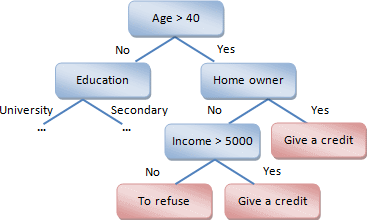
\includegraphics[width=\textwidth]{decisionTree}
\caption{Decision tree about choosing whether to give credit to someone or not}
\label{fig:decisionTree}
\end{figure}
		 
\paragraph{Artificial Neural Networks}
	
The artificial neural networks are one of the widely employed tools in the machine learning. They simulate the learning and predicting activity of the brain. Similar to the process of teaching humans, the artificial neural nets are trained with pairs of data - input variable and their corresponding result value according to the task. Then the net should be able to guess the output value of random input value that wasn't part of the training set. \\\\The  fundamental part of an artificial neural network is the model of the neuron. It consists of three elements\cite{haykin2009neural}:
\vspace{-\topsep}
\begin{enumerate}
\item set of synapses. Each synapse has a weight $w_{kj}$.  When passing through the synapse, the input signal $x_j$ is multiplied by its weight. The weight can hold positive and negative values.
\item an adder. Sums the multiplied input signals. 
\item an activation function. The sum of the adder's value and the bias $b_k$ goes as its argument. The function returns the output signal of the neuron. Its purpose is to restrict the output signal between specific values e.g. -1 and 1.
\end{enumerate}
\vspace{-\topsep}

\begin{figure}[h]
\centering
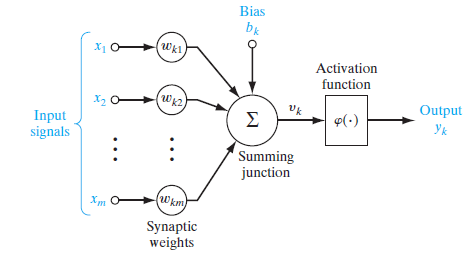
\includegraphics[width=\textwidth]{neuronModel}
\caption{Model of the artificial neuron $k$. Source: \cite{haykin2009neural}}
\label{fig:neuronModel}
\end{figure}

\hspace{1cm}\\ A scheme of the model could be seen on \hyperref[fig:neuronModel]{Fig. \ref{fig:neuronModel}}. Mathematically the neuron $k$ could be described with the following equations:

\begin{equation}
u_k = \sum_{j=1}^{m} w_{kj}x_j
\end{equation}

\begin{equation}
v_k = u_k + b_k
\end{equation}

\begin{equation}
y_k = φ(v_k)
\end{equation}Shortly explained the multiplication of all input signals $x_j$ with the weights $w_{kj}$ of their synapses are getting summed. This sum is then biased with $b_k$ and the result is put into the activation function $φ(.)$, which produce the output signal $y_k$.\\\\
The are some possibilities for activation function, but the mostly used are the sigmoid functions. A sigmoid function has a \enquote{S} shaped graph and and returns value from 0 to 1 or from -1 to 1. One example is the logistic function.
\begin{equation}
φ(v) = \frac{1}{1 + exp(e^{-x})}
\end{equation}
One particular reason why the sigmoid functions are mostly employed as activation functions is the fact that they are differentiable. This quality is later important for the backpropagation. \\\\The simplest neural net consists from only one neuron. Further, we can have many neurons in one single layer. In that  case the net is called single-layer feedforward network. If the net consists from more than one layer, then it's called multilayer feedforward network. Multilayer networks have an input layer, an output layer and could also have a hidden layer or many of them. The ones with many hidden layers are called deep networks\cite{haykin2009neural}.

\begin{figure}[h]
\centering
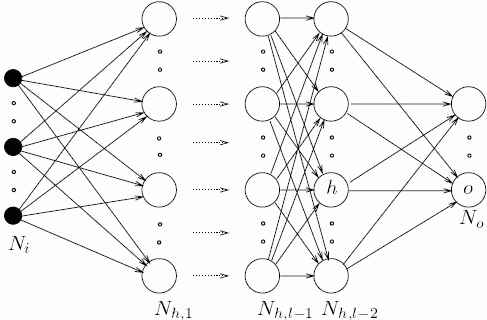
\includegraphics[width=\textwidth]{deepNetwork}
\caption{Schema of deep network: Source: \url{http://www.codeproject.com/KB/cs/BackPropagationNeuralNet/fig1_nnet_thinner.png}}
\label{fig:deepNetwork}
\end{figure}  
  
\hspace{1cm}\\ The ultimate goal of training each neural network is the adjusting of all weight values in such a way that by passing an unknown input signal to the network, it will return a correct output signal. In order to achieve that, a technique called backpropagation is used. Simply explained, we need to pass an input signal through the network. Then we calculate the difference between the real expected value and the output value. With a special loss function and the difference as argument we calculate the new weight for each synapse and then adjust it by propagating the network backwards\cite{rumelhart1986learning}.\\\\ In order to employ the backpropagation the model have to fulfil two conditions. First, the activation function must be differentiable. The logistic function fulfils that. Second, there has to be no addition of $u_k$ with the bias, but at the same time the effect of the bias must be kept. That's achieved by using an extra dummy synapse with weight $w_{k0} = b_k$ and an input signal equals 1 or -1\cite{haykin2009neural}.
		 \paragraph{Ensemble Techniques}
In machine learning and statistics, combining forecasts from different models are recognised as one of the most successful approaches to prediction tasks and are used to obtain better predictive performance, to enhance accuracies and produce overall improved results. 
%(e.g. Dietterich (2000); Brown and Kuncheva (2010))
\\\\However, forecast combination is a challenging task. 
The idea is to find a suitable hypothesis that will make adequate predictions for a particular problem. Ensemble methods are essentially strategies for creating multiple hypotheses and combining them to generate a better hypothesis. This usually produces more accurate solutions than a single hypothesis would. Using adequate ensemble techniques guarantees aggregation of the forecasting strengths, diminution of their weaknesses and efficient error reduction.\\\\There is a recent suggestion that there is an ideal number of component classifiers called \enquote{the law of diminishing returns in ensemble construction}. 
%(https://www.researchgate.net/profile/Hamed_R_Bonab)
Because the number of component classifiers has a high impact on the accuracy of the prediction, having more or less than this ideal number would deteriorate the accuracy. \\\\We distinguish one ensemble approach from another by the way they manipulate the training data, by the way of selection of individual hypotheses and by the way in how those are aggregated to the final decision. 
%Chapter 13 ensemble methonds
In this particular section we will cover some commonly used ensemble approaches, namely Bagging, AdaBoost and Stacking(ref).

\subsubsection{1. Bagging}
%chapter 13 cite all refferences.
\hspace{1cm}\\\\This method is introduced by Breiman [ref] and is used for training each learner with the help of a bootstrap sample from a training set S and then combining each output by uniform averaging. To generate each individual predictor, no information about the predictions of the other models is integrated. For this particular reason this technique is viewed as an algorithm with only an implicit search for diversity. By averaging a set of predictors which are not trained by the same bootstrap sample, there might be a reduction of the influence of the outliers [ref]. Taking that into consideration, resampling seems to have a similar effect to that of robust M-estimators in statistics [ref],  meaning the influence of sample points is restricted using suitable loss functions. Therefore, it is possible that this approach will significantly reduce the variance of the bagged prediction, especially for unstable base learners [ref]. \\\\Because of the fact that traditional bootstrap breaks the sequence of data points, there is a possibility for a bad generalization in time series problems. Inoue and Kilian adjust to the situation by adapting the way that Bagging construct its training samples [ref]. In order to simultaneously capture the reliance between the examples and to encourage diversity,  the authors have to use resampling blocks of instances from the original training set with replacement. This process is called \enquote{block bootstrap}, and the block size is chosen to capture the dependence in error term [ref].
\\\\Bagging, according to a simulation study,  significantly reduces the out-of-sample mean squared error of the predictions. By giving a weight for each example that resemble the number of times the point is selected in the bootstrap sample, the training samples in ...[ref] maintain the temporal arrangement of the points. In this manner, an example is weighted to zero if it has not been selected in the sample. Conclusively, the output of the ensemble for a single instance is computed as a weighted average, where the weight of each predictor is the weighted root mean squared error (WRMSE). [ref]

\subsubsection{2. AdaBoost}
%chapter 13 cite all ref
\hspace{1cm}\\\\This method is introduced by Freud and Schapire in 1997 [ref]. The idea is to train a single predictor to minimize the residual of the previous ensemble in each round, which can be described as a sequentially coupled approach fitting an additive model through a forward stagewise strategy [ref]. The theoretical background of the algorithm is based on the \enquote{PAC} learning model [59] and its purpose is to create a method that combines a set of weak learners to generate a strong learning algorithm. This approach offers good generalization ability, but on the other hand, because of the fact that the learners are coupled sequentially it is computationally expensive. \\\\Maintaining a sampling distribution over the training set is the main purpose behind AdaBoost. With the start of the algorithm, all weights are set to $w^1_m = 1/N, m = 1,..., M$. Here,  $w^n_m$ is the weight of the $m$-th example at round $n$.  The weak learner is forced to focus on the misclassified examples of the training set at each round of the algorithm, because of the specific way in which the weights of the incorrectly classified examples are increased. Hence, instead of focusing on the correctly classified examples, the algorithm concentrates on the \enquote{hard} examples, making it possible for AdaBoost to outperform Bagging in normal scenarios. Nevertheless, under noisy data the low generalization capacity of AdaBoost makes the robustness of Bagging generally superior. \\\\ In the field of time series, Shresta and Solomatine introduce AdaBoost.RT [61]. Here the absolute relative error (ARE) for the learner $n$ is computed by considering the error over a threshold $φ$. The weights of the instances with errors lower than $φ$ are reduced by the updating rule, and afterwards normalized in order to make them a distribution. Conclusively, F is obtained as the weighted average of the individual learners, with weights equal to - $log(β_n)$. \\\\For tide levels forecasting, Canestrelli uses Drucker's AdaBoost.R2(62).  This approach quantifies the loss for each training sample with the help of one of the three possible functions: 
\begin{enumerate}
\item Absolute percentage error (APE):
\begin{equation}
φ(v) = \frac{|f_n(x_m)-y_m|}{max_{m=1,...,M} |f_n(x_m)-y_m|}
\end{equation}
\item Quadratic:
\begin{equation}
w^n_m = (f_n(x_m)-y_m)^2 max_{m=1,...,M} (f_n(x_m)-y_m)^2
\end{equation}
\item Exponential:
\begin{equation}
1 - exp\frac{-|f_n(x_m)-y_m|}{max_{m=1,...,M} |f_n(x_m)-y_m|}
\end{equation}
\end{enumerate}

\hspace{1cm}\\\\According to the weight distribution, the confidence of the predictor is computed as a function of the weighted average error. In order to increase their chances to appear in the following training sample, the instances with higher errors increase their weights. Then the output of the ensemble is computed as the weighted median. \\\\ For recurrent neural networks as the base learner, Assaad et al. adapts this method [63]. The following changes are present: first, the example errors are weighted for updating the RNN weights instead of resampling. The motivation behind this is to keep the temporal dependence of the training data. Second, the weight of the wrong modeled examples is further increased using an additional parameter. \\\\ As an adaptation of AdaBoost.R2 technique with Genetic Programming (GP) as the base learner, Souza et al. [64] proposes the BCC algorithm. This essentially computes the error of each example with the help of the exponential loss function.  And by including a multiplicative factor which depends on the correlation among the learner predictions and the true targets, the algorithm updates the weights. \\\\ Finally, as a combination of Ellman Newtorks using a weighted linear function, Goh et al. [65] introduces the Modified AdaBoost. On top of that, the error of each instance is computed by taking into account two loss functions. These are widely used for analysing drug dissolution profiles. [chapter 13] \\\\ The goal of AdaBoost, according to the gradient descent perspective of AdaBoost [8,66], is to add the i-th learner in the ensemble which minimizes
\begin{equation}
(β_n, f_n)=argmin_{(β,f)} \sum_{m=1}^{M} l(y_m, F(x_m)).
\end{equation}
Here $F(x_m)=F_{n-1}(x_m)+ β_n f_n (x_m)$. With each following step, the algorithm selects the hypothesis $f_n$ which minimizes Eq. (8) over the sample distribution $w^n$. Then it performs a line search along the direction. From this perspective, Buhlmann and Yu [67] introduce a gradient boosting method with the quadratic loss function which is adapted for time seies forecasting for load forecasting [68], finance [69], economics [70] and production [71].

\subsubsection{3. Stacking}
\hspace{1cm}\\\\ Stacking, also known as stacked generalization, first introduced by David H. Wolpert [?] in 1992, is a strategy for minimizing the generalization error rate of one or more generalizers. The method works by deducting the biases of the generalizers with respect to a provided learning set. For instance, it uses the guess of the original generalizers as input (when taught with part of the learning set and trying to guess the rest of it) and the correct guess for output. The difference between using multiple generalizers and using a single generalizer is that in the first case, stacked generalization can be considered as a more sophisticated version of cross-validation for it exploits a better strategy than cross-validation's crude winner-takes-all [?] for combining the individual generalizers. In the second case, when used with a single generalizer, stacked generalization is a schema for estimating the error of a generalizer, trained on a particular learning set and then asked a particular question. \\\\Stacking has a distinguishing feature and that is that the information fed up the net of generalizers comes from multiple partitionings of the original set, feeding information from one set of generalizers to another, then making the final guess. Each of these generalizers splits up that learning set into two subsets. Collecting information about the biases of the generalizing behaviour of the original generalizers with respect to the learning set is the purpose of these pairs of subsets. This collected bias information is the one fed up the net. One can conclude that stacked generalization, as a means of estimating and correcting for the biases of the constituent generalizers with respect to the corresponding learning set, can be expected to reduce the generalization error rate for many generalization problems, according to the experiments done in [?].
		 
		\subsubsection{General time series forecasting methods}
\paragraph{Linear}
One way to forecast the value of an observation $x_t$ using previous observations is to use linear stochastic difference equation models, with random input. Without any doubt the linear autoregressive integrate moving average (ARIMA) model is the most important class of such models. The seasonal ARIMA $(p, d, q) × (P, D, Q)^S$ model for such time series is represented by
\begin{equation}
Φ_P (B^S)φ_p(B)∇^D_S ∇^d x_t = Θ_Q(B^S)θ_q (B)ε_t.
\end{equation}
Here $φ_P (B^S)$ is the nonseasonal autoregressive operator of order p, $θ_q (B)$ is the nonseasonal moving average operator of order q, $Φ_P (B^S), Θ_Q(B^S)$ are the seasonal autoregressive and moving average operator of order P and Q. The terms $x_t$ and $ε_t$ are the time series and a white noise, respectively. Additionally it is assumed that $E[ε_t|x_{t−1}, x_{t−2},...] = 0$. This condition is satisfied for example when $ε_t$ are
zero mean, identically distributed and independent of past $x_ts$. It is assumed throughout that $ε_t$ has finite variance $σ^2$. The backshift operator B shifts the index of a time series observation backwards,  e.g. $Bx_t = x_{t−1}$ and $B^k x_t = x_{t−k}$. Akaike’s information criterion (AIC) or by Bayes information criterion (BIC) [8] select the order of the operator and the parameters $Φ_1,...,Φ_P , φ_1,...,φ_p, Θ_1,...,Θ_Q$ and $θ_1,...,θ_q$ are selected from the time series data using optimization methods such as maximum likelihood [1] or  robust methods such as recursive generalized maximum likelihood [9]. The system generating the time series must be invariant and stable, which means that the ARMA-models is limited by the requirement of stationarity and invertibility of the time series. Moreover, the residuals must be independent and identically distributed [10]. \\\\In order to be useful for predictions, the ARMA-models require a stationary time series. Therefore, for all $t$:
\begin{equation}
E[x_t] = μ; \quad V[x_t] = σ^2; \quad COV[x_t, x_{t−k} ] = γ_k 
\end{equation}
for a series to be weak stationary.
\\\\Some of the most popular tests for diagnostic checking of the overall ARMA models are the \enquote{portmanteau test} proposed by [11] and the robust version of it by [12]. The tests are based on a sum of squared correlations of the estimated residuals suitably scaled. [chapter 13]. 
\paragraph{Non-linear}
There has been increasing interest in non-linear models recently. The reason for that being that while theory and practice are mostly concerned with linear methods and models (like ARIMA), many time series exhibit features, which cannot be explained in a linear framework. Bilinear models [13], classification and regression trees [14], threshold autoregressive models [15] and Projection Pursuit Regression [16] are all great examples for non-linear models. Although non-linear models can be substantial in some instances, it is usually challenging to compute forecasts more than one step ahead [17]. \\\\ As a generalization of the linear ARMA-models to the non-linear case, proposed by [18], NARMA follows the equation
\begin{equation}
x_t = h(x_{t−1}, x_{t−2},..., x_{t−p}, ε_{t−1},...,ε_{t−q} ) + ε_t .
\end{equation}
Here $h$ is an unknown smooth function and, as earlier described, it is assumed that $E[ε_t|x_{t−1}, x_{t−2},...] = 0$ and that variance of $ε_t$ is $σ^2$. In this case the conditional mean predictor based on the infinite past observation is
\begin{equation}
x'_t = E[h(x_{t−1}, x_{t−2},..., x_{t−p}, ε_{t−1},...,ε_{t−q} )|x_{t−1}, x_{t−2},...]. 
\end{equation}
We assume the invertibility of the NARMA model in the sense that there exists a function $ν$ such as
\begin{equation}
x_t = ν(x_{t−1}, x{t−2}, . . .) + ε_t . 
\end{equation}
Then given the infinite past of observations $x_{t−1}, x_{t−2},...,$ one can compute the $ε_{t−1}$ in (11) exactly:
\begin{equation}
ε_{t−j} = κ(x_{t− j}, x_{t− j−1}, . . .), j = 1, 2,..., q. 
\end{equation}
In this case the mean estimate is
\begin{equation}
x'_t = h(x_{t−1}, x_{t−2},..., x_{t−p}, ε_{t−1},...,ε_{t−q} ).
\end{equation}
Here the $ε_{t− j}$ are specified in terms of present and past $x_u$’s. The predictor of (15) has a mean square error $σ^2$. We cannot compute (14) and (15) due to the finite observation record. It makes sense to approximate the conditional mean predictor (15) by the recursive algorithm
\begin{equation}
x'_t = h(x_{t−1}, x_{t−2},..., x_{t−p}, ε'_{t−1},..., ε'_{t−q} ), 
\end{equation}
\begin{equation}
ε'_{t− j} = x_{t− j} − x'_{t− j}, j = 1, 2,..., q,
\end{equation}
with the following initial conditions
\begin{equation}
x'_0 = x'_{−1} =...= x'_{−p+1} = ε'_0 =...= ε'_{−q+1} = 0. 
\end{equation}
For the special case of non-linear autoregressive model (NAR), it is easy to check that (11) is given by
\begin{equation}
x_t = h(x_{t−1}, x_{t−2},..., x_{t−p}) + ε_t .
\end{equation}
In this case, the minimum mean square error (MSE) optimal predictor of $x_t$ given $x_{t−1}, x_{t−2},..., x_{t−p}$ is the conditional mean (for $t ≥ p + 1$).
\begin{equation}
x'_t = E[x_t|x_{t−1},..., x_{t−p}] = h(x_{t−1},..., x_{t−p}).
\end{equation}
This predictor has mean square error $σ^2$.
\paragraph{Concept Drift}
Concept drift refers to the fact that data is obtained form a non-stationary environment [19] and it means that the underlying law of probability changes regarding the time series. It can be described as any scenario in the classification setting, where the posterior probability of  a class $c_k$ to which a given instance belongs, $P(C_k|x)= P(x|c_k)P(c_k)/P(x)$, changes over time as follows: $P_{t+1}(c_k|x)≠ P_t(c_k |x)$. $P(x)$ represents probability of an instance  $x ∈ X$. $P(c_k|x)$ is the likelihood of observing a data point $x$ within a particular class. $P(c_k)$ defines the class prior probabilities and relates class balance to the overall underlying law of probability. An observation of change in $P(x)$ is independent of the class labels. For that reason it might be insufficient to characterize a concept drift. \\\\ There exist two ways of adapting a model to a concept drift. The first approach is to adapt a single model so that it can learn example by example and adapt to a changing pattern. The second approach is to create an ensemble of models. According to Zang et al. [20], both examples have the same capacity to handle stream data, with the inclusion of a concept drift. While in terms of efficiency the incremental single algorithms are favourable, the ensembles are more stable and better-adapting to the concept drift.	
\section{Arbitrated Ensemble for Time Series Forecasting} In this section we will present a relatively new method for time series forecasting, which by far gives the most accurate results in comparison to older state-of-the-art methods. It was introduced by a team of Portuguese scientists on the European Conference on Machine Learning that took place on 18-22 September 2017 in Skopje, Macedonia. 

\subsection{General explanation}
\vspace{-\topsep}
Many forecasting methods use combination of different forecasters in order to achieve better accuracy by reducing the overfitting effect. So does the method of arbitrated ensemble as well. It assumes that every forecaster has its own expertise and has to be as diverse as possible. Due to the volatility and the seasonality of time series this unique expertise isn't equally distributed over time - some forecasters are more accurate at specific time (more precisely with input data with specific characteristics), other forecasters - at other specific time. Hence, we must build an ensemble of forecasters by first weighting them according to their expertise on the specific situation and second - summing the products of each forecaster and its expertise weight \cite{VtorCerqueira2017}. \\\\That leads us to the second essence of the presented method - the arbitrating, also known as arbitrating architecture. To arbitrate means in our case to decide how important is each forecaster for the final prediction. This happens through a second level of forecasters called meta-learners. Each main forecaster (or learner) has its own meta-learner. The meta-learner predicts the possible error of its learner according to the current input data characteristics. Those error values are later  translated to forecaster's weights using  softmax function. The greater the predicted error is, the less the weight of the forecaster will be \cite{VtorCerqueira2017}.
\vspace{-\topsep}

\begin{figure}[h]
\centering
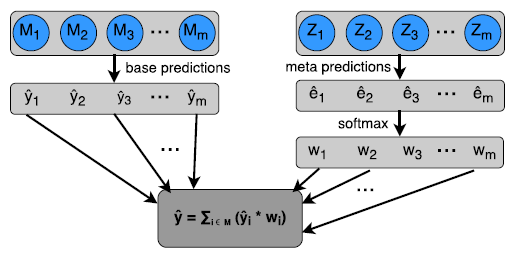
\includegraphics[width=\textwidth]{adeSchema}
\caption{Schema of the Arbitrated Dynamic Ensemble (ADE). $M_1, ... ,M_m$ are the main forecasters. They produce the predictions $y_1, ... ,y_m$. The meta-forecasters $Z_1, ... ,Z_m$ predict the error values $e_1, ... ,e_m$ of each main forecaster. From those errors the expertise weights $w_1, ... ,w_m$ are generated. At last the weights are used to calculate the weighted average of the predictions. \cite{VtorCerqueira2017}}
\label{fig:adeSchema}
\end{figure} 
 
\vspace{-\topsep}
\hspace{1cm}\\ The above described process is called Arbitrated Dynamic Ensemble (ADE) by its authors. It's illustrated on \hyperref[fig:adeSchema]{Fig. \ref{fig:adeSchema}}. 

\subsection{Data preparation and Learning Basic-Level Models}
Time series is generally a temporal sequence of values. In our case $Y={y_1,y_2,...,y_t}$. Here $y_i$ is the value of $Y$ at time $i$. To represent Y in an Euclidean space with embedding dimension K, time delay embedding is used. Now we have produced a set of observation which are based on the past $K$ lags of the time series. This is accomplished by mapping the time series $Y$ into the embedding vectors $V_{N-K+1} = {v_1,v_2,...,v_{N-K+1}}$. Here each $v_i =\ <y_{i-(K-1)},y_{i-(K-1)},...,y_i>$. \\\\ Three main steps are essential for the proposed methodology in ADE for time series prediction:
\begin{enumerate}
\item An offline training step of $M$, the set of base-learners which are used to predict future values of $Y$ and the online iterative steps.
\item Training or updating of meta-learners Z, which model the expertise of base-learners.
\item Prediction on $y_{i+1}$ using $M$, dynamically weighed according to Z.
\end{enumerate}
Individual forecasters $m$ are trained in the offline learning phase [Algo1]. Each $M^j, ∀j ∈ {1,...,m}$ is built using the available time series $Y^K_{tr}$. The goal is the prediction of the next value of the series, $y_{t+1}$. Training and testing sets are named $tr$ and $ts$, correspondingly. \\\\ In order to apply standard regression learning models, we have to embed the time series to an Euclidean space. Then $M$ is comprised by a set of heterogeneous models, like for example Neural Networks and Gaussian Processes. Such models provide different inductive biases and assumptions regarding the process generating the data. Therefore, it is expected models to differentiate in competence across the time series.

\begin{algorithm}[h]

\caption{Learning $M$}\label{alg:learning}
\begin{algorithmic}[1]

\Require Available Time Series $Y$; Embedding Dimension $K$
\State $\text{Embed $Y$ into $Y_{tr}^{K}$}$
\ForAll{$M^j \in M$}
\State $\text{train $M^j$ using $Y_{tr}^K$}$
\EndFor
\State $\text{Return $M$}$
\end{algorithmic}
\end{algorithm}

\subsection{Learning Meta-Level Models}
The layer of meta-learners or meta-forecasters has to be trained to arbitrate the importance of each learner for the current prediction. As it was already mentioned, each learner has its own expertise. The task of the learner's corresponding meta-learner is to measure its expertise for a specific situation. In order to do that it has to predict the estimated error of the learner for that situation. The  described strategy is based on an arbitrating architecture, which was originally used with classifies and not with regression forecasters \cite{ortega2001arbitrating}. We train the meta-learner by using data samples corresponding to the following model:\begin{equation}
e^j = f(I)
\end{equation} $e^j$ is the absolute error caused by $M^j$, $I$ are the past values of the time series and $f$ is the regression function.\\\\ At the training phase our first task is to produce the out-of-bag predictions (OOB). We will than use them to train the meta-learners once before the start of the actual prediction session and once every time after predicting $y_t+1$. So, to produce the OOB we split the training set into $\beta$ equal blocks. We train the learners $M$ with the first block of data and then test them with the second. Then we merge the first and the second block, train the learners with this new larger block and test them with the third block. The operation continues up to the last block.\\\\Instead of using all base learners by predicting, it's a common sense to use only the best of them. We call the used learners the Committee of Models for Prediction. It contains the $\alpha$\% of the best forecasters (the one with the lowest error) in the last $\Omega$ observations. This reduction saves computational power from retraining of meta-learners that have learners with very low weight. Nevertheless, no matter whether its base learner is part of the committee of models or not, each meta-learner is trained on each $\lambda$ iterations. You can see the meta-learning algorithm in \hyperref[alg:metalearning]{Algorithm  \ref{alg:metalearning}}.
    
\begin{algorithm}[h]

\caption{Metalearnig $Z$}\label{alg:metalearning}
\begin{algorithmic}[1]

\Require Available observations at runtime $Y_{ts}$; Embedding Dimension $K$; Training
Signal $\lambda$; meta-committee ${}^{\alpha}Z$
\State $\text{Embed $Y_{ts}$ into $Y_{ts}^{K}$} \rightarrow I$
\ForAll{$Z^{j} \in {}^{\alpha}Z \text{ and not trained in the last training signal $\lambda$ }$}
\State $\text{train $Z^{j}$ to model: $e^{j} = f(I)$}$
\EndFor
\State $\text{Return ${}^{\alpha}Z$}$
\end{algorithmic}
\end{algorithm}

\subsection{Predicting the next time series}
 After the Committee of the most accurate $\alpha$\% base learners ${}^{\alpha}M$  is determined, we use the corresponding meta-learners ${}^{\alpha}Z$ to predict their possible error $e^j$. Then we put these errors into the softmax function and thus we generate the base learner's weighs\cite{VtorCerqueira2017}. This process is explained by the following equation:
 \begin{equation}
w^{j}_{t+1} = \frac{exp(-e^{j})}{\sum_{j \in {}^{\alpha}M} exp(-e^{j})}
\end{equation} It's interesting fact the the softmax function is used for neural nets modelling. Even more, it wasn't used by far for error translation.\\\\ The last step of the prediction is the calculation of the weighted average by summing the products of all predictions of the committee with their weights:
 \begin{equation}
y_{t+1} = \sum_{j \in {}^{\alpha}M} y^{j}_{t+1}.w^{j}_{t+1}
\end{equation}You can see the predicting $y_{t+1}$ algorithm in \hyperref[alg:predicting]{Algorithm  \ref{alg:predicting}}.


\begin{algorithm}[h]
\caption{Predicting $y_{t+1}$}
\label{alg:predicting}
\begin{algorithmic}[1]
\Require $K, M, Z,\alpha, \Omega, {}^{\alpha}M, {}^{\alpha}Z$
\State $\text{Embed the previous $K-1$ values  into $Y_{t+1}^{K}$}$
\State $\text{Get meta-predictions $e^{j}_{t+1}$ from $Z^{j} \in {}^{\alpha}Z$}$
\State $\text{Compute weigths $w^{j}_{t+1} =  exp(-e^{j}_{t+1})/\sum_{Z^{j} \in {}^{\alpha}Z} exp(-e^{j}_{t+1})$}$
\State $\text{Get predictions $y^{j}_{t+1} $ from models $M^{j} \in {}^{\alpha}M$}$
\State $\text{Compute final predictions $y_{t+1} = \sum_{j=1}^{m} y^{j}_{t+1}.w^{j}_{t+1}$}$
\State $\text{Add $y_{t+1}$ to $Y_{ts}$}$
\State $\text{Update Committees ${}^{\alpha}M$ and ${}^{\alpha}Z$ according to $\alpha$ and $\Omega$}$
\State $\text{Return $y_{t+1}$ and go back to the metalearning step (Algorithm \ref{alg:metalearning})}$
\end{algorithmic}
\end{algorithm}

\subsection{Performance comparison with general time series forecasting methods}
In order to highlight the benefits of the arbitrated dynamic ensemble (ADE) method performance-wise versus other state-of-the-art methods for time series prediction tasks, we will take a look at the experiments [paper] performed to validate ADE. In the following subsections we will cover the setup, the results, strategies and limitations.
\subsubsection{Experimental Setup}
\hspace{1cm}\\\\ The mean squared error (MSE) is used to evaluate the used methods on 10 Monte Carlo repetitions. Then for each one of these repetitions, a randomly chosen point in time is set from the full time window available for each series. The previous window $N$ consists of 50\% of the data set and the following window consists of 30\%. They are used for training the ensemble and testing, respectively. For comparison between the results collected by the different methods, the non-parametric Wilcoxon Signed Rank test was used. The experiments were carried out with the help of performanceEstimation [28] R package. In addition to that, two different embedding dimensions were tested by setting K to 7 and 15. 
\subsubsection{Ensemble Setup and Baselines}
\hspace{1cm}\\\\ In this experiment, the following base-models $M$ were present:
\begin{itemize}
\item SVM: Support Vector Machines [15];
\item NN: Feed Forward Neural Nets [29];
\item GP: Gaussian Processes [15];
\item GLM: Generalized Linear Models [11];
\item RF: Random Forests [31];
\item GBR: Generalized Boosted Regr. [24];
\item MARS: MARS [18];
\item RBR: Rule-based Regression [16];
\item PPR: Projection Pursuit Regr. [23].
\end{itemize}
Each of the individual learners is used with different parameter settings, which helps to add up to 40 models. Also Random Forest is used as a meta-learner. The meta-learners are retrained every 10 observations. Up to the upcoming prediction, each set contains the out-of-bag (OOB) samples from the training set and the observations from the test set. Only half of the forecasters are included in the committee for each prediction, namely the forecasters with the best performance in the last 50 observations. \\\\ The following 8 approaches were compared against the performance of ADE: 
\begin{itemize}
\item Stacking: An adaptation of stacking [30] for time series, where a meta-model is learned using the base-level predictions as attributes; 
\item Arbitrating: The original arbitrating approach [21];
\item S: A static heterogeneous ensemble. All base learners are simply averaged using the arithmetic mean [26];
\item S-W: A weighted linear combination of the models, with weights according to their performance using all past information [14];
\item AEC: The adaptive combination procedure AEC [25];
\item S-WRoll: The adaptive combination method with a linear combination of the forecasters according to their recent performance [19];
\item ERP: The adaptive combination procedure proposed by Timmermann [27];
\item ARIMA: A state-of-the-art method for time series forecasting;
\end{itemize}
The following variants of ADE (with Random Forest as a meta-learner) were tested:
\begin{itemize}
\item ADE-Arb: A variant of ADE in which at each time point the best model is selected to make a prediction. The one with lowest predicted loss is the best;
\item ADE-meta-runtime: A variant of ADE in which there is no blocked prequential procedure to obtain OOB samples to increase the data provided to the meta-learners. In this scenario $Z$ is trained in data obtained only at run-time;
\item ADE-all-models: A variant of ADE, but without the formation of a committee. In this case, all forecasting models are weighed according to their expertise in the input data;
\item ADE-linear-committee: A variant of ADE, but using a linear transformation for weighting the base learners according to their predicted loss instead of the proposed softmax;
\item ADE-meta-GP: A variant of ADE, but using a Gaussian Process with a linear kernel as meta-learner instead of a Random Forest;
\end{itemize}
\subsubsection{Results}
\hspace{1cm}\\\\ In the following Figure [6] are presented the paired comparisons between the proposed method, ADE, and the baselines. The proposed method shows significantly more wins and losses. 

\begin{figure}[h]
\centering
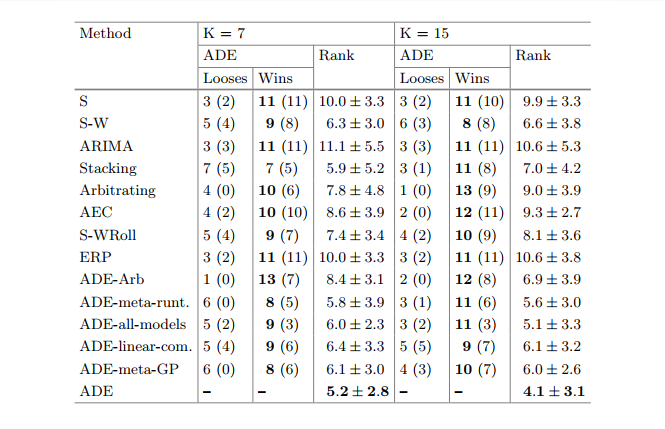
\includegraphics[width=\textwidth]{pairedComparison}
\caption{Paired comparisons between the proposed method and the baselines for different embedding dimensions. The Rank column stands for the average rank and respective standard deviation of each model. A rank of 1 in the
experiment means that the model was the best method.}
\label{fig:paired comparison}
\end{figure}

\hspace{1cm}\\\\ The post-hoc Bonferroni-Dunn test corresponding to the other baselines in the literature and baselines which are variants of ADE are to be seen in the critical difference diagrams (Figure [7] and Figure [8], respectively).

\begin{figure}[h]
\centering
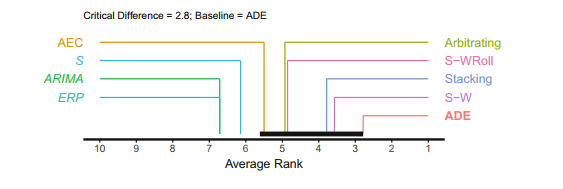
\includegraphics[width=\textwidth]{criticalDifference1}
\caption{Critical difference diagram for the post-hoc Bonferroni-Dunn test relative to baselines (K = 7).}
\label{fig:critical difference diag.1}
\end{figure}

\begin{figure}[h]
\centering
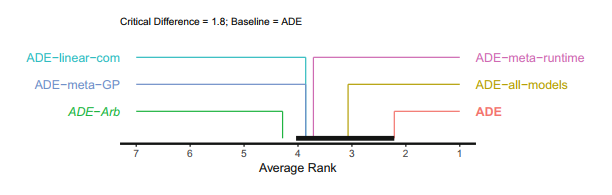
\includegraphics[width=\textwidth]{criticalDifference2}
\caption{Critical difference diagram for the post-hoc Bonferroni-Dunn test relative to ADE variants (K = 7).}
\label{fig:critical difference diag.2}
\end{figure}

\hspace{1cm}\\\\ These results display the performance of ADE in comparison to the state-of-the-art approaches for time series forecasting tasks. In relation to the meta-learning layer, using Random Forests generated better results than Gaussian Processes. Against meta-learning strategies for combining models such as Stacking there aren't any significant differences other than a better average rank. In connection to Arbitrating, ADE shows a much better average rank, proving that the introduced components are fundamental for the accomplished performance. Therefore, it is more beneficial to use a weighing scheme in our Arbitrating strategy instead of choosing the predicted best forecaster as originally proposed [21]. Because of the consistent advantage of ADE over ADE-meta-runtime and ADE-all-models, we can conclude that it is very beneficial to get OOB predictions from the training set to increase the data used to train the meta-learners, improving their fit and cutting down the ensemble for each prediction. This means the introduction of a committee is really favourable. Relative to the ADE-linear-committee, the proposed method shows that the softmax function provides a superior predictive performance in comparison to the linear transformation. Against ADE-Arb, according to Figure 7 and 8, the difference is statistically significant. 

\subsubsection{Training Strategies}
\hspace{1cm}\\\\ Another aspect that has to be considered is how the performance of ADE can vary in dependence of the updating strategy for the base and meta-models. In the paper [ref] are examined the following approaches:
\begin{itemize}
\item A: $M$ are not updated and $Z$ are updated in chunks of $\lambda$ observations;
\item B: $M$ and $Z$ are both trained only in the training set;
\item C: $M$ and $Z$ are both re-trained every $\lambda$ observations;
\item D: $M$ is re-trained every $\lambda$ observations but $Z$ is trained only in the training data.
\end{itemize}
These strategies are compared using the mean absolute scaled error (MASE):
\begin{equation}
\frac{\sum^n_{i=1}|e_i|}{\frac{n}{n-1} \sum^n_{i=2}|y_i-y_{i-1}|}
\end{equation}
The results of this test are in the following Figure [9]. The figure displays the average MASE and average runtime and corresponding deviations of ADE using the different re-training strategies.

\begin{figure}[h]
\centering
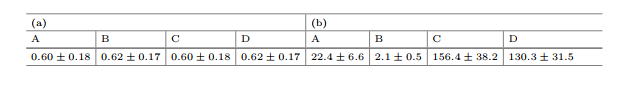
\includegraphics[width=\textwidth]{trainingStrategies}
\caption{ Average MASE and respective deviation of the different retraining strategies in terms of predictive performance (a) and computational time spent in minutes (b).}
\label{fig:training Strategies}
\end{figure}

\hspace{1cm}\\\\
The results conclude that updating the meta-learners and not updating the base-learners (A) (both in predictive performance and runtime) is better than the opposite strategy (D).

\subsubsection{Limitaions}
\hspace{1cm}\\\\ While the advantages of the proposed method are evident and its performance is competitive with the commonly used stacked generalization method [30], ADE has also limitations. One of them is the inability to directly model inter-dependencies among the forecasters. Another is the fact that base-learners might get outdated, but thanks to the modular architecture of the arbitration approach, models can be added (or removed) as required.

\section{Conclusion}

\subsubsection{Acknowledgments}

%%%%%%%%%%%%%%%%%%%%%%%%%%%%%%%%%%%%%%%%%%%%%%%%%%%%%%%%%%%%%%%%%%%%%%%%%%%%%%%
\bibliographystyle{splncs03}
\bibliography{paper}

%%%%%%%%%%%%%%%%%%%%%%%%%%%%%%%%%%%%%%%%%%%%%%%%%%%%%%%%%%%%%%%%%%%%%%%%%%%%%%%

\end{document}
